\documentclass[main.tex]{subfiles}
\begin{document}

\chapter{Topologische Grundbegriffe}


\section{Topologische Räume}

\begin{Definition}[Topologie]
  Ein \textbf{topologischer Raum} ist ein geordnetes Paar $(X,\tau)$ bestehend aus einer Menge $X$ und einer Familie von Teilmengen $\tau$ von $X$, die den folgenden 3 Axiomen genügt.

  \begin{minipage}[t]{0.5\textwidth}
    \begin{enumerate}
      \item $\emptyset \subseteq X$ ist offen und $X \subseteq X$ ist offen.
      \item Beliebige Vereinigungen von offenen Mengen sind offen.
      \item Endliche Durchschnitte von offenen Mengen sind offen.
    \end{enumerate}
  \end{minipage}
  \begin{minipage}[t]{0.5\textwidth}
    \begin{enumerate}
      \item $\emptyset, X \in \tau$
      \item $U_1, U_2 \in \tau \Rightarrow U_1 \cap U_2 \in \tau$
      \item $\mathcal{U} \subseteq \tau \Rightarrow \bigcup_{U \in \mathcal{U}} U \in \tau$
    \end{enumerate}
  \end{minipage}

  Wir nennen die Familie $\tau$ eine \textbf{Topologie} auf $X$ und Teilmengen $U \subseteq X$, die zur Familie $\tau$ gehören \textbf{offene} Mengen.

  Wir nennen...
  \begin{itemize}
    \item eine Teilmenge $F \subseteq X$, deren Komplement offen ist, eine \textbf{abgeschlossene} Teilmenge.
    \item eine Teilmenge $V \subseteq X$ \textbf{Umgebung} von $x$, falls eine offene Teilmenge $U \subseteq X$ mit $x \in U$ und $U \subseteq V$ existiert.
    \item eine Teilmenge $V$ eine \textbf{offene Umgebung} von $x$, falls $V$ offen ist.
    \item eine Teilmenge $V$ eine \textbf{abgeschlossene Umgebung} von $x$, falls $V$ abgeschlossen ist.
  \end{itemize}
\end{Definition}

\begin{Beispiel}
  \begin{itemize}
    \item $\mathcal{P}(X)$ für eine Beliebige Menge $X$ ist eine Topologie. Sie heißt diskrete Topologie auf $X$, bezüglich ihr sind alle Teilmengen von $X$ offen. (Sie sind alle in $\tau$ enthalten.)
    \item $\tau = \{\emptyset,X\}$ ist ebenfalls eine Topologie, nämlich die triviale, oder indiskrete Topologie.
    \item Die Klasse aller Mengen, die jeweils nur $x$ enthalten, für alle Elemente aus $X$ definiert eine Topologie auf $X$.
  \end{itemize}
\end{Beispiel}

\begin{Definition}[Induzierte Topologie]
  Sei $X$ ein topologischer Raum, sei $Y \subseteq X$ eine Teilmenge. Wir nennen
  $$\tau|_Y = \{Y \cap U \mid U \subseteq X \text{ offen }\}$$
  die auf $Y$ \textbf{induzierte Topologie}. ($U$ offen $\Leftrightarrow U \in \tau$)

  $V \subseteq Y$ ist offen (für die induzierte Topologie) genau dann wenn eine offene Teilmenge $U \subseteq X$ existiert, mit $V = Y \cap U$. Allgemeiner nennen wir in diesem Fall $V \subseteq Y$ \textbf{relativ offen}.
\end{Definition}

\begin{Beispiel}
  $X = \R^3$, $Y = \{(x,y,z) \mid x^2 + y^2 + z^2 = 1 \}$ (die Kugeloberfläche).

  Hier wird (selbstverständlicherweise) die Standardtopologie verwendet. Diese Teilmenge $Y \subseteq X$ ist nicht offen (es lassen sich keine offenen Bälle um alle Punkte legen).

  Bezüglich anderer Topologien kann die Antwort anders ausfallen.
  $$V = \{(x,y,z) \mid x^2 + y^2 + z^2 = 1, z > 0 \}$$
  ist in $Y$ offen, in $X$ aber weiterhin nicht, also relativ offen.

  Beweis: $V = Y \cap \underbrace{\{(x,y,z) \mid z > 0\}}_{\text{offen in } \R^3}$
\end{Beispiel}

\begin{Definition}[Umgebung]
  Sei $X$ ein topologischer Raum, $x \in X$. Eine Teilmenge $W \subseteq X$ heißt \textbf{Umgebung} von $x$, falls eine Teilmenge $U \subseteq X$ existiert mit $x \in U \subseteq W$.

  Ist $W$ offen, so ist $W$ eine Umgebung von $x$.
\end{Definition}

\begin{Definition}
  Sei $X$ ein topologischer Raum, $Y \subseteq X$.
  \begin{itemize}
    \item Das \textbf{Innere} von $Y$ ist
      $$\begin{aligned}
        \mathring{Y} &= \{x \in Y \mid Y \text{ ist eine Umgebung von } x\}\\
        &= \{x \in Y \mid \E U \in x \text{ offen mit } x \in U \subseteq Y\}
      \end{aligned}$$
      \begin{Bemerkung}[Alternative Definition]
        $$\bigcup_{\substack{U \text{ offen} \\ U \subseteq Y}} U = \left( \overline{Y^C}\right)^C$$
      \end{Bemerkung}
      \begin{Theorem}
        $$\mathring{Y} \text{ ist offen.}$$
      \end{Theorem}
    \item Der \textbf{Abschluss} von $Y$ ist
      $$\overline{Y} = \{x \in X \mid W \cap Y \neq \emptyset \A \text{ Umgebungen } W \text{ von } x\}$$
      \begin{Bemerkung}[Alternative Definition]
        $$\overline{Y}= \left(\mathring{(Y^C)}\right)^C = \bigcap_{\substack{A \text{ abgeschlossen} \\ \text{mit } Y \subseteq A}} A$$
      \end{Bemerkung}
      \begin{Lemma}
        Sei $(X,\tau)$ ein topologischer Raum, $Y \subseteq M \subseteq X$ Unteraume und $\tau_M$ eine induzierte Topologie.

        Für $\overline{Y^M}$, den Abschluss von $Y$ bezüglich $M$ gilt:
        $$\overline{Y^M} = \overline{Y} \cap M$$
      \end{Lemma}
    \item Der \textbf{Rand} von $Y$ ist
      $$\partial Y = \overline{Y} \backslash \mathring{Y} = X \backslash \left(\mathring{Y} \cup (\mathring{Y})^C\right)$$
  \end{itemize}
\end{Definition}

\begin{Beispiel}
  $X = \R$, $Y = (0,1]$. Dann gilt:
  $$\mathring{Y} = (0,1) \quad \overline{Y} = [0,1] \quad \partial Y = \{0,1\}$$
\end{Beispiel}

\begin{Beweis}[der Äquivalenz der Definitionen von Abschluss]
  $$\begin{aligned}
    x \in \mathring{(Y^C)} & \Leftrightarrow \E U \text{ offen }: x \in U \text{ und } U \cap Y \neq 0 \\
    x \notin \mathring{(Y^C)} & \Leftrightarrow \A U \text{ offen }: x \in U \text{ und } U \cap Y \neq 0 \\
    & \Leftrightarrow x \in \left(\mathring{(Y^C)}\right)^C
  \end{aligned}$$
\end{Beweis}

\begin{Beweis}[des Lemmas]
  $$\begin{aligned}
    & x \in M \cap \overline{Y^M} \\
    \Leftrightarrow & \E U \in \tau : x \in U \text{ und } U \cap Y = \emptyset \text{ und } x \in M \\
    \Leftrightarrow & x \in U \cap M \text{ und } (U \cap M) \cap Y = \emptyset \\
    \Leftrightarrow & x \in \left(\overline{Y^M}\right)^C \\
    \Rightarrow & \overline{Y^M} = \overline{Y} \cap M
  \end{aligned}$$
\end{Beweis}


\subsection{Stetige Abbildungen}

\begin{Definition}[Homöomorphismus]
  Seien $(X,\tau)$ und $(X,\sigma)$ topologische Räume. Eine \textbf{stetige Abbildung} von $(X,\tau)$ nach $(X,\sigma)$ ist eine Abbildung $f: X \to Y$ so, dass für jede offene Teilmenge $U \subseteq Y$ das Urbild $f^{-1}(U) \subseteq X$ offen ist.

  Eine bijektive, stetige Abbildung, deren Inverses ebenfalls stetig ist, heißt \textbf{Homöomorphismus}.
\end{Definition}

\begin{Theorem}
  Seien $X$, $Y$ und $Z$ topologische Räume.
  \begin{itemize}
    \item Die Identitätsabbildung $id_X : X \to X$ ist stetig.
    \item Sind $f: X \to Y$ und $g: Y \to Z$ stetig, so ist die Verknüpfung $g \circ f : X \to Z$ ebenfalls stetig.
    \item Ist $f : X \to Y$ stetig und bijektiv, so ist die Umkehrabbildung $f^{-1}: Y \to X$ im Allgemeinen \textbf{nicht} stetig.
  \end{itemize}
\end{Theorem}

\begin{Theorem}
  Sei $D \subseteq \R$ eine Teilmenge, und $f: D \to \R$ eine Funktion. Die folgenden Aussagen sind äquivalent:
  \begin{enumerate}
    \item Für jedes $x_0 \in \R$ und jedes $\varepsilon > 0$ existiert ein $\delta > 0$ so, dass
      $$|x - x_0| < \delta \Rightarrow |f(x) - f(x_0)| < \varepsilon \A x \in D$$
    \item Für jede offene Teilmenge $U \subseteq \R$ ist $f^{-1}(U) \subseteq D$ offen, für die von der Standardtopologie auf $\R$ induzierten Topologie auf $D$.
  \end{enumerate}
\end{Theorem}

\begin{Beweis}
  Siehe Skript.
\end{Beweis}

\subsection{Folgenkonvergenz in topologischen Räumen}

\begin{Definition}
  Sei $X$ ein topologischer Raum, $(x_n)_{n=0}^\infty$ eine Folge un $X$.
  \begin{itemize}
    \item Ein Punkt $a \in X$ heißt \textbf{Grenzwert} der Folge $(x_n)_{n=0}^\infty$, falls:
      $$\A \text{ Umgebung } W \text{ von } a \E N \in \N : x_n \in W \A n > N$$
    \item Ein Punkt $a \in X$ heißt \textbf{Häufungspunkt} der Folge $(x_n)_{n=0}^\infty$, falls:
      $$\A \text{ Umgebung } W \text{ von } a \A N \in \N : \E n \geq N : x_n \in W$$
  \end{itemize}
\end{Definition}

\begin{Definition}[Hausdorff'sche topologische Räume]
  Ein topologischer Raum $X$ heißt \textbf{Hausdorff'sch}, falls für alle $x,y \in X$ mit $x \neq y$ Umgebungen $w$ von $x$ und $V$ von $y$ existieren mit
  $$W \cap V = \emptyset$$
\end{Definition}

\begin{Beispiel}
  \begin{itemize}
    \item Die Standardtopologie ist Hausdorff'sch.
    \item Jeder metrische Raum, als Topologie aufgefasst, ist Hausdorff'sch.
  \end{itemize}
\end{Beispiel}

\begin{Theorem}
  Sei $X$ ein Hausdorff'scher topologischer Raum, $(x_n)_{n=0}^\infty$ eine Folge in $X$. Dann hat $(x_n)_{n=0}^\infty$ höchstens einen Grenzwert $a \in X$. Wir schreiben
  $$a = \limn x_n$$
\end{Theorem}

\begin{Beweis}
  Seien $x$ und $y \in X$ Grenzwerte von $(x_n)_{n=0}^\infty$. Sei $V$ eine Umgebung von $x$, $U$ eine Umgebung von $y$. Dann existiert $N \in \N$, so dass:
  $$n \geq N \Rightarrow x_n \in V$$
  $$n \geq N \Rightarrow x_n \in U$$
  Daraus folgt, dass $U \cap V \neq 0$, also laut der Definition des Hausdorff'schen Raums: $x = y$.
\end{Beweis}

\begin{Definition}[Folgenstetigkeit]
  Eine Abbildung $F: X \to Y$ zwischen Hausdorff'schen topologischen Räumen heißt \textbf{folgenstetig} falls für jede konvergente Folge $(x_n)_{n=0}^\infty$ in $X$ mit $\limn x_n = x$ und $\limn f(x_n)_{n=0}^\infty = f(x)$.
\end{Definition}

\begin{Bemerkung}[Warnung]
  $$\begin{array}{c c c}
    \text{stetig} & \Rightarrow & \text{folgenstetig} \\
    & \not\Leftarrow &
  \end{array}$$
\end{Bemerkung}

\subsection{Topologie und metrische Räume}

\begin{Theorem}
  Jeder metrische Raum induziert eine Topologie.
\end{Theorem}

\begin{Beispiel}[Veranschaulichung]
  Sei $(X,d)$ ein metrischer Raum. Die von $d$ induzierte Topologie hat als offene Mengen, Mengen der Form $U$ mit
  $$\A x \in U \E \varepsilon > 0 : B_\varepsilon(x) \subseteq U$$
\end{Beispiel}


\section{Kompaktheit}

\begin{Definition}[Überdeckung]
  Sei $X$ ein topologischer Raum. Eine \textbf{offene Überdeckung} von $X$ ist eine Familie offener Mengen $(U_i)_{i \in \mathcal{I}}$ mit $U_i \subseteq X$ offen, so dass
  $$\bigcup_{i \in \mathcal{I}} U_i = X$$
  gilt.

  Wir sagen, dass für eine Teilmenge $\mathcal{J} \subseteq \mathcal{I}$ die Familie $(U_j)_{j \in \mathcal{J}}$ eine \textbf{Teilüberdeckung} ist, falls
  $$\bigcup_{j \in \mathcal{J}} U_j = X$$
  gilt. Wir nenn diese Überdeckung \textbf{endlich}, falls $\mathcal{J}$ endlich ist.
\end{Definition}

\begin{Beispiel}
  Die Menge aller offenen Teilmengen von $X$ ist eine Überdeckung.

  Die Menge $X$ ist eine Überdeckung von $X$.
\end{Beispiel}

\begin{Definition}[Kompaktheit]
  Ein topologischer Raum $X$ heißt \textbf{kompakt}, falls \textbf{jede} offene Überdeckung von $X$ eine endliche Teilüberdeckung hat.
\end{Definition}

\begin{Bemerkung}
  Dies kann in der Regel von Hand nicht nachgeprüft werden, wir brauchen also andere Werkzeuge.
\end{Bemerkung}

\begin{Beispiel}[Gegenbeispiele]
  \begin{itemize}
    \item $X = \R$. Setze $U_n = B(n, 1) = (n-1,n+1)$. Jetzt ist $(U_n)_{n \in \Z}$ ist eine offene Überdeckung, hat aber offensichtlich keine endliche Teilüberdeckung.

      $\Rightarrow \R$ ist nicht kompakt.
    \item $X = (0,1) \subseteq \R$. Setze $U_n = \left(\frac{1}{n}, 1- \frac{1}{n}\right)$ für $n \geq 3$
      $$\bigcup_{n=3}^\infty U_n = (0,1) = X$$
      hat keine endliche Teilüberdeckung.

      $\Rightarrow (0,1)$ ist nicht kompakt. (Wir zeigen später, dass aber $[0,1]$ es ist.)
  \end{itemize}
\end{Beispiel}

\begin{Bemerkung}
  Ist $X$ ein topologischer Raum, so heißt $A \subseteq X$ kompakt, falls $A$ als eigenständiger topologischer Raum (mit der von $X$ induzierten Topologie) kompakt ist.

  Das heißt: $A$ ist kompakt, wenn für jede Familie offener Mengen $(U_i)_{i \in \mathcal{I}}$ in $X$ mit
  $$A \subseteq \bigcup_{i \in \mathcal{I}} U_i$$
  eine endliche Teilmenge $\mathcal{J} \subseteq \mathcal{I}$ existiert mit:
  $$A = \bigcup_{j \in \mathcal{J}} U_j$$
\end{Bemerkung}

\begin{Theorem}[Schachtelungsprinzip]
  Sei $X$ ein topologischer Raum. Dann ist $X$ kompakt genau dann, wenn das folgende \textbf{Schachtelungsprinzip} gilt:

  Sei  $\mathcal{A}$ eine Familie abgeschlossener Teilmengen von $X$, so dass
  $$A_1 \cap A_2 \cap ... \cap A_n \neq \emptyset$$
  für alle $A_n \in \mathcal{A}$. Dann gilt:
  $$\bigcap_{A \in \mathcal{A}} A \neq \emptyset$$
\end{Theorem}

\begin{Beweis}
  \begin{itemize}
    \item kompakt $\Rightarrow$ Schachtelung

      Sei $\mathcal{A} = (A_i)_{i \in \mathcal{I}}$ eine Familie abgeschlossener Teilmengen von $X$ mit
      $$\bigcap_{i \in \mathcal{I}} A_i = \emptyset$$
      Setze $U_i = X \backslash A_i \subseteq X$ offen. Es gilt
      $$\bigcap_{i \in \mathcal{I}} U_i = X$$
      $X$ kompakt: $\E \mathcal{J} \subseteq \mathcal{I}$ endlich mit
      $$\bigcup_{j \in \mathcal{J}} U_j = X \Leftrightarrow \bigcap_{j \in \mathcal{J}} A_j = \emptyset$$
    \item Schachtelung $\Rightarrow$ kompakt

      In die andere Richtung lesen.
  \end{itemize}
\end{Beweis}

\begin{Korollar}
  Ist $X$ kompakt und $A \subseteq X$ abgeschlossen, so ist $A$ kompakt.
\end{Korollar}

\begin{Theorem}
  Sei $f: X \to Y$ eine stetige Abbildung zu topologischen Räumen, und sei $A \subseteq X$ kompakt.

  Dann ist $f(A) \subseteq Y$ kompakt.
\end{Theorem}

\begin{Beweis}
  Sei $(U_i)_{i \in \mathcal{I}}$ eine Familie offener Mengen in $Y$ mit
  $$f(A) \subseteq \bigcup_{i \in \mathcal{I}} U_i$$
  $f$ ist stetig $\Rightarrow V_i := f^{-1}(U_i) \subseteq X$ ist offen. Es gilt
  $$A \subseteq \bigcup_{i \in \mathcal{I}} V_i$$
  Es existiert $\mathcal{J} \subseteq \mathcal{I}$ endlich mit
  $$A \subseteq \bigcup_{j \in \mathcal{J}} V_j$$
  $$\Rightarrow f(A) \subseteq \bigcup_{j \in \mathcal{J}} U_j$$
\end{Beweis}


\begin{Definition}[Folgenkompaktheit]
  Ein topologischer Raum $X$ heißt \textbf{folgenkompakt}, falls jede Folge $(x_n)_{n=0}^\infty$ in $X$ eine konvergente Teilfolge besitzt.

  Ein metrischer Raum $(X.d)$ heißt (folgen)kompakt, falls $X$ als topologischer Raum ($\tau$ von $d$ induziert) (folgen)kompakt ist.
\end{Definition}

\begin{Definition}[Beschränktheit von metrischen Räumen]
  Ein metrischer Raum $(X,d)$ heißt \textbf{beschränkt}, falls
  $$\E R > 0 : d(x,y) \leq R \A x,y \in X$$
  Wir nennen $(X,d)$ \textbf{total beschränkt} falls für jedes $r > 0$ endlich viele $x_1, ..., x_n \in X$ existieren, mit
  $$X = \bigcup_{k=1}^n B(x_k,r)$$
\end{Definition}

\begin{Bemerkung}
  Insbesondere sind kompakte Intervalle total beschränkt.
\end{Bemerkung}

\begin{Definition}[Lebesgue-Zahl]
  Sei $(X,d)$ ein metrischer Raum, $(U_i)_{i \in \mathcal{I}}$ eine offene Überdeckung von $X$. Eine reelle Zahl $\lambda > 0$ heißt \textbf{Lebesgue-Zahl} zu dieser Überdeckung, falls für alle $x \in X$ ein $i \in \mathcal{I}$ existiert, mit $B(x,\lambda) \subseteq U_i$.
\end{Definition}

\begin{Beispiel}
  Sei $X = \R^2$. Betrachte:
  $$U_1 = \{(x,y) \mid y > 0 \}$$
  $$U_2 = \{(x,y) \mid y < \exp(-x)\}$$
  \begin{center}
    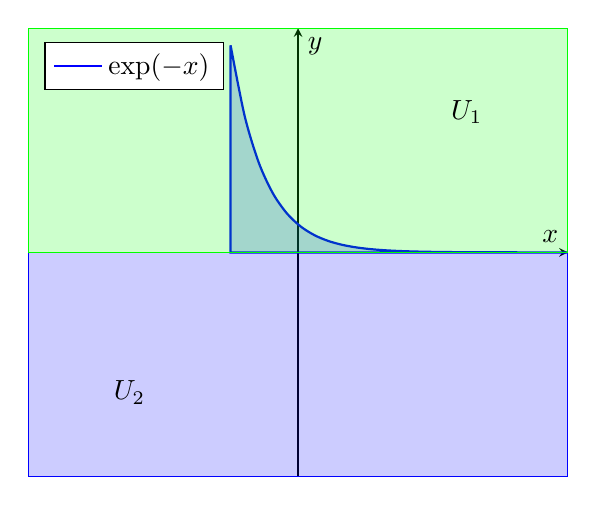
\begin{tikzpicture}
      \begin{axis}[
        domain=-8:8,
        ymin=-8,ymax=8,
        axis x line = center,
        ticks=none,
        axis y line = center,
        xlabel={$x$},
        ylabel={$y$},
        legend pos=north west,
      ]
        \addplot[domain=-2:8,smooth,thick,blue,fill,fill opacity=0.2] {e^(-x)} \closedcycle;
        \addplot[smooth,blue,fill,fill opacity=0.2] {-8} \closedcycle;
        \addplot[smooth,green,fill,fill opacity=0.2] {8} \closedcycle;
        \addlegendentry{$\exp(-x)$}
        \node at (5, 5)   (a) {$U_1$};
        \node at (-5, -5)   (b) {$U_2$};
      \end{axis}
    \end{tikzpicture}
  \end{center}

  Eine Lebesgue-Zahl existiert hier nicht.
\end{Beispiel}


\begin{Theorem}
  Sei $X$ ein \textbf{metrischer Raum}. Die folgenden Aussagen sind äquivalent:
  \begin{enumerate}
    \item $X$ ist kompakt.
    \item $X$ ist folgenkompakt.
    \item Jede unendliche Teilmenge von $X$ hat einen Häufungspunkt.
    \item Jede stetige, reellwertige Funktion $f: X \to \R$ ist beschränkt.
    \item Jede stetige Funktion $f: X \to \R$ nimmt ihr Maximum und Minimum auf $X$ an.
    \item $X$ ist total beschränkt und jede offene Überdeckung von $X$ besitzt eine Lebesgue-Zahl.
    \item $X$ ist total beschränkt und vollständig.
  \end{enumerate}
\end{Theorem}

\begin{Bemerkung}
  Diese Aussagen ergeben im Allgemeinen nur für metrische Räume einen Sinn, für topologische Räume können wir diese Aussagen gar nicht erst treffen; sie setzen eine Metrik voraus. (Beispielsweise Cauchy-Folgen.)
\end{Bemerkung}

\begin{Beweis}[Vorausschau]
  \begin{itemize}
    \item[$I$] $(3) \Rightarrow (2) \Rightarrow (7) \Rightarrow (3)$
    \item[$II$] $(4) \Leftrightarrow (5) \Leftrightarrow (3)$
    \item[$III$] $(6) \Rightarrow (1) \Rightarrow (3) (\Rightarrow (5)) \Rightarrow (6)$
  \end{itemize}
\end{Beweis}
Umsetzung:

\begin{Beweis}[Teil $I$]
  \begin{itemize}
    \item $(3) \Rightarrow (2)$

      Sei $(x_n)_{n=0}^\infty$ eine Folge in $X$. Betrachte $D = \{x_n \mid n \geq 0\}$. Ist $D$ endlich, so hat $(x_n)_{n=0}^\infty$ eine konstante Teilfolge, also einen Häufungspunkt. Ist $D$ unendlich, so hat $D$ einen Häufungspunkt $a \in X$.

      Behauptung: $a$ ist Häufungspunkt der Folge $(x_n)_{n=0}^\infty$.

      Sei $\varepsilon > 0$, $N \in \N$ und zeige:
      $$\E n \geq N : d(a,x_n) < \varepsilon$$
      Wähle $\varepsilon' \leq \varepsilon$ und $d(x_k,a)>\varepsilon'$ für alle $k = 0,1,2,...,N$ mit $x_k \neq a$.

      \incfig{d_unendlich}
      \begin{center}
        $D \cap B(a, \varepsilon')$ ist undenlich.
      \end{center}

      $\E n \in \N$ mit $x_n \in B(a,\varepsilon')$ und $x_n \neq a$. Dann muss $n \geq N$. Also $\E n \geq N : d(a, x_n) < \varepsilon' < \varepsilon$.
    \item $(2) \Rightarrow (7)$

      $X$ vollständig: Sei $(x_n)_{n=0}^\infty$ eine Cauchy-Folge in $X$. Nach Voraussetzung hat diese Folge einen Häufungspunkt und konvergiert also. (Jede Folge, die eine konvergente Teilfolge hat, konvergiert.)

      $X$ total beschränkt: $A\!\!\!A$ Angenommen, $X$ sei nicht total beschränkt:
      $$\E r > 0 : \A \text{ endliche Teilmenge } F \subseteq X : \bigcup_{x \in F} B(x, r) \subsetneq X$$
      Wähle $x_0 \in X$, wähle $x_1 \in X \backslash B(x_0, r)$. Verfahre $n$-Mal analog: $x_n \in X \backslash (B(x_0,r) \cup B(x_1,r) \cup ... \cup B(x_{n-1, r}))$ Die Folge $(x_n)_{n=0}^\infty$ hat keinen Häufungspunkt, weil $\A n > m \geq 0 : d(x_n, x_m) > r$. Also gilt $(2)$ nicht: \lightning
    \item $(7) \Rightarrow (3)$

      Sei $D \subseteq X$ unendlich. Wir konstruieren eine Cauchy-Folge in $D$ mit paarweise verschiedenen Gliedern. Der Grenzwert dieser Folge ist dann ein Häufungspunkt von $D$.

      $X$ ist toal beschränkt: $\E F_0 \subseteq X$ endlich mit
      $$X = \bigcup_{x \in F_0} B(x, 1)$$
      Es existiert $y_0 \in F_0$ mit $D_0 = D \cap B(y_0, 1)$ unendlich.

      Es existiert auch $F_1 \subseteq X$ ebenfalls endlich mit
      $$X = \bigcup_{x \in F_1} B(x, 2^{-1})$$
      Es existiert $y_1 \in F_1$ mit $D_0 = D \cap B(y_1, 2^{-1})$ unendlich.
      $$\begin{array}{c | c | c | c}
        \hline
        y_0 & D_0 = B(y_0,1) \cap D & unendlich & x_0 \in D_0 \\
        \hline
        y_1 & D_1 = B(y_1,2^{-1}) \cap D_0 & unendlich & x_1 \in D_1 \\
        \hline
        y_2 & D_2 = B(y_2,2^{-2}) \cap D_1 & unendlich & x_2 \in D_2 \\
        \hline
          & ... & ... &
      \end{array}$$
      $$d(x_0,x_1) \leq 1 \quad d(x_1,x_2) \leq \dfrac{1}{2} \quad d(x_2,x_3) \leq \dfrac{1}{4} \quad ... \quad d(x_n,x_m) \leq 2^{-n+1}$$
      Die Folge $(x_n)_{n=0}^\infty$ ist Cauchy.
  \end{itemize}
\end{Beweis}

\begin{Beweis}[Teil $II$]
  \begin{itemize}
    \item $(4) \Rightarrow (5)$ (Die Rückrichtung ist offensichtlich)

      Sei $f: X \to \R$ stetig. Setze $M = \sup\{f(x) \mid x \in X\}$. $A\!\!\!A$ Angenommen $f(x) < M \A x \in X$. Dann gilt:
      $$g(x) = \dfrac{1}{M - f(x)} \text{ ist wohldefiniert und stetig auf} X$$
      $g$ ist nach Voraussetzung beschränkt, also $\E S \in \R : g(x) \leq S \A x \in X$
      $$\begin{aligned}
        f(x) & \leq M - \dfrac{1}{S} \\
        \Leftrightarrow \sup \{f(x) \mid x \in X\} & \leq M - \dfrac{1}{S} \\
        & < M = \sup \{f(x) \mid x \in X\}
      \end{aligned}$$
      $$\Rightarrow -\dfrac{1}{S} = 0 \Leftrightarrow -1 = 0 \lightning$$
    \item $(5) \Rightarrow (3) (\Leftrightarrow \lnot (3) \Rightarrow \lnot (5))$

      Angenommen $D \subseteq X$ sei unendlich und ohne Häufungspunkte. Sei $\eta : X \to \R$ die Funktion
      $$\eta (x) = \sup \{\delta > 0 \mid |B(x, \delta) \cap D| \leq 1 \}$$
      Die Menge $D$ hat keine Häufungspunkte also gilt $\eta (x) > 0 \A x \in X$.

      Behauptung: $\eta$ ist stetig. Seien $x_1, x_2 \in X$. Setze $r = \eta (x_1) - d(x_1,x_2)$. Falls $r > 0$, dann gilt:
      $$B(x_2,r) \subseteq B(x_1n\eta(x_1))$$
      Folgt: $\eta (x_2) \geq r = \eta (x_1) - d(x_1,x_2)$ (gilt trivialerweise auch für $r \leq 0$). Besser gesagt:
      $$|\eta(x_1) - \eta(x_2)| \leq d(x_1, x_2) \quad \text{aus Symmetrie}$$
      $$\Rightarrow \eta \text{ stetig}$$

      Aus $(5)$ folgt außerdem: $\E r > 0 : \eta(x) \geq r \A x \in X$.

      Sei $x_0,x_1,...$ eine Folge verschiedener Elemente aus $D$. Definiere $f: X \to \R$ durch:
      $$f(x) = \left\{\begin{array}{c c c}
        n \cdot \left(\frac{1}{4} r - d(x,x_n)\right) & \text{falls} & x \in B\left(x_2,\frac{r}{4}\right) \\
        0 & \text{sonst} &
      \end{array}\right.$$
      \incfig{disjunkte_baelle}
      Die Funktion $f$ ist stetig aber nicht beschränkt: $f(x_n) = \frac{1}{4} r \cdot n$

      $(3) \Rightarrow (5)$

      \adabs $f: X \to \R$ sei nach oben unbeschränkt und stetig. Es existiert für $n \in \N$ ein $x_n \in X$ mit $f(x_n) \geq m$. Die Folge $(x_n)_{n=0}^\infty$ hat keinen Häufungspunkt.

      Hätte sie einen, so hätte sie eine konvergente Teilfolge. $f$ angewandt auf diese konvergente Teilfolge ergäbe wieder eine konvergente Folge. Diese wäre per Voraussetzung aber nicht beschränkt. \lightning
  \end{itemize}
\end{Beweis}

\begin{Beweis}[Teil $III$]
  \begin{itemize}
    \item $(6) \Rightarrow (1)$

      Sei $(U_i)_{i \in \mathcal{I}}$ eine offene Überdeckung von $X$.
      $$(\E \lambda > 0 : \A x \in X \E i \in \mathcal{I} : B(x ,\lambda) \subseteq U_i)$$
      Es existieren endlich viele $x_1, ..., x_n$ mit:
      $$X = \bigcup_{k = 1} B(x_k, \lambda)$$
      Wähle $i_k \in \mathcal{I}$ mit $B(x_{k_i}, \lambda) \subseteq U_{i_k}$. Dann gilt:
      $$X = \bigcup_{k = 1} U_{i_k}$$
    \item $(1) \Rightarrow (4) \Leftrightarrow (2),(5)$

      Sei $f: X \to \R$ stetig.
      $$X = \bigcup_{n = 1}^\infty \underbrace{f^{-1}((-n,n))}_{offen}$$
      Aus $(1)$ folgt $X = f^-1((-n,n))$ für ein $n \in \N$ (groß genug).
      $$\Rightarrow f \text{ beschränkt}$$
    \item $(2),(5) \Rightarrow (6)$

    Existenz eine Lebesgue-Zahl.

    Sei $(U_i)_{i \in \mathcal{I}}$ eine offene Überdeckung von $X$. Betrachte $\eta : X \to \R$ gegeben durch:
    $$\eta(x) = \sup \{\delta > 0 \mid \E i \in \mathcal{I} \text{ mit } B(x,\delta) \subseteq U_i \}$$
    Es gilt $\eta(x) > 0 \A x \in X$. Die Funktion $\eta$ ist stetig.

    Nach $(5)$ gilt dann: $\eta(x) \geq r$ für ein $r > 0$. Dann ist $\lambda = \frac{r}{2}$ eine Lebesgue-Zahl.

    Angenommen $X$ sei nicht total beschränkt: $\E r > 0$, so dass $X$ nicht eine Vereinigungen endlich vieler Bälle mit Radius $r$ ist. Wähle rekursiv:
    $$x_0 \in X \quad x_1 \in X \backslash B(x_0,r) \quad ... \quad x_n \in X \backslash (B(x_0,r) \cup ... \cup B(x_{n-1},r))$$
    Die Folge $(x_n)_{n=0}^\infty$ hat keinen Häufungspunkt, da $d(x_n,x_m) \geq r \A n \neq m$
  \end{itemize}
\end{Beweis}

\begin{Theorem}
  Seien $X$, $Y$ metrische Räume und $f: X \to Y$ stetig. Ist $X$ kompakt, so ist $f$ gleichmäßig stetig.
\end{Theorem}

\begin{Beweis}
  Sei $\varepsilon > 0$. Es genügt, ein $\delta > 0$ zu konstruieren, dass die Bedingung der gleichmäßigen Stetigkeit erfüllt:

  Da $f$ stetig ist, existiert für jedes $x \in X$ ein $\delta_x > 0$ mit
  $$d(x,x') < \delta_x \Rightarrow d(f(x),f(x')) < \dfrac{\varepsilon}{\color{olive} 2}$$
  also auch:
  $$f(B(x,\delta_x)) \subseteq B\left(f(x),\frac{\varepsilon}{\color{olive} 2}\right)$$
  Es gilt:
  $$X = \bigcup_{x \in X} B\left(x,\frac{\delta_x}{2}\right)$$
  ist eine offene Überdeckung von $X$.

  $X$ kompakt:$\E x_1, ..., x_n \in X$ mit
  $$X = \bigcup_{i = 1}^n B\left(x,\frac{\delta_{x_i}}{2}\right)$$
  Setze $\delta := \min \left\{ \frac{\delta_{x_1}}{2},\frac{\delta_{x_2}}{2},...,\frac{\delta_{x_n}}{2} \right\}$

  Überprüfe, dass $\delta$ der Voraussetzung genügt:

  Seien $x,x' \in X$ mit $d(x,x') < \delta$. Also $\E i \in \{1,...,n\}$ mit $x \in B(x_i,\frac{\delta_{x_i}}{2})$. Dann gilt $x' \in B(x_i,\delta_{x_i})$.
  $$\begin{aligned}
    d(f(x),f(x')) & \leq d(f(x),f(x_i)) + d(f(x_i),f(x')) \\
    & \leq \dfrac{\epsilon}{2} + \dfrac{\varepsilon}{2} = \varepsilon
  \end{aligned}$$
\end{Beweis}

\begin{Theorem}
  Sei $X$ ein metrischer Raum, $A \subseteq X$ eine Teilmenge.
  $$A \text{ kompakt } \Rightarrow A \textbf{ beschränkt } \text{und} \textbf{ abgeschlossen}$$
\end{Theorem}

\begin{Beweis}
  Nach dem vorherigen Satz (Teil $(1) \Leftrightarrow (7)$) ist $A$ total beschränkt (also insbesondere beschränkt) und vollständig. Sei $(x_n)_{n = 0}^\infty$ eine Folge in $A$, $x \in X$ mit $x = \limn x_n$. Da $(x_n)_{n = 0}^\infty$ konvergiert ist die Folge Cauchy, also existiert $a \in A$ mit $a = \limn x_n$. Folgt $a = x \in A$ und somit ist $A$ nach dem Folgenkriterium für Abgeschlossenheit abgeschlossen.
\end{Beweis}

Nun können wir endlich richtig zeigen:
\begin{Theorem}[Heine-Borel]
  Sei $n \geq 0$. Eine Teilmenge $A \subseteq \R^n$ ist kompakt genau dann, wenn $A$ beschränkt \textbf{und} abgeschlossen ist.
\end{Theorem}

\begin{Korollar}
  Abgeschlossene und beschränkte Intervalle sind kompakt.
\end{Korollar}

\begin{Beweis}
  Ist $A$ kompakt, dannn folgt: $A$ beschränkt und abgeschlossen. (siehe oben)

  Ist umgekehrt $A$ beschränkt und abgeschlossen, dann lässt sich zeigen: $A$ ist folgenkompakt $\Leftrightarrow$ kompakt, dank dem obigen Satz.

  Sei $(x_n)_{n = 0}^\infty$ eine Folge in $A$. Diese kann aufgefasst werden als eine Folge im $\R^n$, die beschränkt ist. Die Folge hat also einen Häufungspunkt in $\R^n$, bezeichnet als $x$. Es gilt:
  $$x = \lim \limits_{k \to \infty} x_{n_k}$$
  $(x_{n_k})_{k = 0}^\infty$ ist eine Folge in $A$. Da $A \subseteq \R^n$ abgeschlossen folgt: $x \in A$. Folgt $A$ folgenkompakt $\Leftrightarrow$ $A$ kompakt.
\end{Beweis}

Dieser Satz stellt ein mächtiges Werkzeug für uns dar: Er wird uns bei sehr vielen weiteren Beweisen hilfreich sein:
\begin{Theorem}[Fundamentalsatz der Algebra]
  Jedes nicht-konstante Polynom $f \in \C[T]$ hat eine Nullstelle in $\C$, also $\E z_0 \in \C : f(z_0) = 0$
\end{Theorem}

\begin{Beweis}
  Gilt trivialerweise $f(0) = 0$, so sind wir fertig. Im Folgenden nehmen wir also an, $f(0) \neq 0$. Also
  $$M := 2 |f(0)| > 0$$

  Da $f$ nicht konstant ist, existiert $R \geq 1$ mit $f(z) > M \A z \in \C : |z| > R$.

  Die Menge $A = \{ z\in \C \mid |z|\leq R\}$ ist beschränkt und abgeschlossen, also kompakt (HB).

  Die Funktion $A \to \R$, $z \mapsto |f(z)|$ ist stetig und nimmt also ihr Minimum auf $A$ an:
  $$\E z_0 \in A : |f(z_0)| \leq |f(z)| \A z \in A$$

  Für $z \in \C \backslash A$ gilt:
  $$f(z) \geq M = 2 |f(0)| \geq 2 |f(z_0)|$$
  Also $|f(z)| \geq |f(z_0)| \A z \in \C$.

  Behauptung: $z_0$ ist Nullstelle von $f$.

  Ersetze $f$ durch $f(z - z_0)$ um oBdA. zu sagen: $z_o = 0$. Also $|f(z)| \geq |f(0)| \A z \in \C$.

  Wir müssen zeigen: $f(0) = 0$. $\adabs$ Angenommen, dies sei nicht der Fall: Schreibe
  $$f(T) = a_0 + a_1 T + a_2 T^2 + ... + a_n T^n \quad n = deg(f) \geq 1$$
  mit $a_n \neq 0$ und $a_0 = f(0) \neq 0$. Wir setzen
  $$z = r \cdot e^{i\varphi} = r \cdot \exp(i\varphi) \quad r = |z| > 0, z \neq 0$$
  Also wird $f$ zu
  $$f(z) = a_0 + a_1 \cdot r \cdot e^{i\varphi} + a_2 \cdot r \cdot e^{i 2 \varphi} + ... + a_n \cdot r \cdot e^{i n \varphi}$$
  Sei $l \in \{1,2,...,n\}$ \textbf{minimal} mit $a_l \neq 0$. Für ein fixes $\varphi$ gilt:
  $$\begin{aligned}
    |f(z)| & = |a_0 + a_l \cdot r^l \cdot e^{i l \varphi} | + \mathcal{O}(r^{l+1}) \quad \text{für } r \to 0 \\
    & = |a_0| \cdot \left|1 + \dfrac{a_l}{a_0} \cdot r^l \cdot e^{i l \varphi} \right| + \mathcal{O}(r^{l+1})
  \end{aligned}$$
  Schreibe $\frac{a_l}{a_0} = s \cdot e^{i \psi}$ und wähle $\varphi = \dfrac{-\psi + \pi}{l}$: Dann gilt: $e^{i(l \varphi + \psi)} = e^{i \pi} = -1$.
  $$\begin{aligned}
    |f(z)| = f(r \cdot e^{i \varphi})| & = |a_0| \cdot |1 + s \cdot e^{i \psi} \cdot r^l \cdot e^{i l \varphi}| + \mathcal{O}(r^{l+1}) \\
    & = |a_0| \cdot |1 - s \cdot r^l| + \mathcal{O}(r^{l+1}) \\
    & \leq |a_0| \underbrace{- |a_0| \cdot s \cdot r^l + \mathcal{O}(r^{l+1})}_{< 0 \text{ für } r \to 0} < |a_0| = |f(0)| \lightning
  \end{aligned}$$
\end{Beweis}

\begin{Beispiel}
  Sei $n \geq 0$, $S^n := \{x \in \R^{n+1} \mid ||x|| = 1 \}$

  Sei $f: S^n \to S \to S^n$ stetig und bijektiv. Dann ist $f^{-1}: S^n \to S^n$ stetig.

  Schreibe  $g := f^{-1}$. Sei $U \subseteq S^n$ offen. zeige: $g^{-1}(U)$ ist offen.

  $A = S^n \backslash U$ ist abgeschlossen und beschränkt in $\R^n$. Folgt $f(A) \subseteq \R^n$ ist kompakt und also insbesondere abgeschlossen.

  Also ist $f(U) = g^{-1}$ offen.
\end{Beispiel}


\section{Zusammenhangsbegriffe}

\begin{minipage}[t]{0.5\textwidth}
  \textbf{Topologisch:}
  \begin{Definition}[Zusammenhang]
    Ein topologischer Raum $X$ heißt \textbf{zusammenhängend}, falls $\emptyset$ und $X$ die einzigen Teilmengen von $X$ sind, die offen \textbf{und} abgeschlossen sind.
  \end{Definition}
  Alternativ:
  \begin{Definition}
    $X$ ist zusammenhängend, falls für alle $U_1, U_2 \subset X$ offen, $U_1 \cap U_2 \neq \emptyset$, $U_1 \cup U_2 = X$ gilt:
    $$U_1 = \emptyset \text{ und } U_2 = X \text{ oder } U_2 = \emptyset \text{ und } U_1 = X$$
  \end{Definition}
  \begin{Definition}
    Wir nennen eine Teilmenge $A \subseteq X$ zusammenhängend, falls $A$ als eigenständiger Raum (mit der von $X$ induzierten Topologie) zusammenhängend ist.
  \end{Definition}
  \begin{Definition}
    Eine Teilmenge $A \subseteq X$, die offen und abgeschlossen und zusammenhängend ist, heißt \textbf{Zusammenhangskomponente} von $X$.
  \end{Definition}
\end{minipage}
\begin{minipage}[t]{0.5\textwidth}
  \textbf{Geometrisch:}
  \begin{Definition}[Zusammenhang]
    Ein topologischer Raum $X$ heißt \textbf{zusammenhängend}, falls für alle $x_1,x_2 \in X$ eine stetige Funktion $\gamma : [0,1] \to X$ mit $\gamma(0) = x_1$ und $\gamma(1) = x_2$ existiert. Wir nennen $\gamma$ einen Pfad oder Weg von $x_1$ nach $x_2$.
  \end{Definition}
  \incfig{weg_zusammenhang}
\end{minipage}

\begin{Bemerkung}
  Im Allgemeinen sind diese Aussagen \text{nicht} gleichwertig: Weg-Zusammenhang impliziert Zusammenhang, aber nicht anders herum.
\end{Bemerkung}

\begin{Theorem}
  Sein $X$ ein topologischer Raum, $Y_1, Y_2 \subseteq X$ zusammenhängende Teilmengen mit $Y_1 \cap Y_2 \neq \emptyset$. Dann ist $Y_1 \cup Y_2$ zusammenhängend.
\end{Theorem}

\begin{Beweis}
  Sei $A \subseteq Y_1 \cup Y_2$ offen, abgeschlossen und nicht leer.
  $$\begin{aligned}
    & A \cap Y_1 \subseteq Y_1 & \text{oBdA. } A \cap Y_1 \neq \emptyset \\
    \Rightarrow & A \cap Y_1 = Y_1  & \text{ also } Y_1 \subseteq A \\
    \Rightarrow & A \cap Y_2 \neq \emptyset & A \cap Y_2 \subseteq Y_2 \neq \emptyset \\
    \Rightarrow & Y_2 \subseteq A & \\
    \Rightarrow & A = Y_1 \cup Y_2 &
  \end{aligned}$$
\end{Beweis}

Diese Aussage können wir auch geometrisch formulieren und beweisen:

\begin{Theorem}
  Sei $X$ ein topologischer Raum, $Y_1, Y_2 \subseteq X$ weg-zusammenhängend, $Y_1 \cap Y_2 \neq \emptyset$. Dann ist $Y_1 \cup Y_2$ weg-zusammenhängend.
\end{Theorem}

\begin{Beweis}
  Seien $x_1, x_2 \in Y_1, Y_2$- Gilt $x_1,x_2 \in Y_1$, so existiert ein Weg von $x_1$ nach $x_2$ in $Y_1 \subseteq Y_1 \cup Y_2$.

  Analog, wenn $x_1, x_2 \in Y_2$.

  Falls $x_1 \in Y_1, x_2 \in Y_2$, dann wähle $x_3 \in Y_1 \cap Y_2$. Sei $\gamma_1$ ein Pfad in $Y_1$ von $x_1$ nach $x_3$ und $\gamma_2$ ein Pfad in $Y_2$ von $x_2$ nach $x_3$.

  Setze
  $$ \gamma(t) = \left\{ \begin{array}{c c c}
    \gamma_1(2t) & \text{ für } & 0 \leq t \leq \frac{1}{2} \\
    \gamma_2(2t - 1) & \text{ für } & \frac{1}{2} \leq t \leq 1
  \end{array}\right.$$
  Dasd ist ein wohldefinierter Pfad von $x_1$ nach $x_2$.
\end{Beweis}

\begin{Theorem}
  Eine Teilmenge $X \subseteq \R$ ist zusammenhängend genau dann, wenn $X$ ein Intervall ist.
\end{Theorem}

\begin{Beweis}
  Falls $X = \emptyset$ \checkmark. Also wählen wir $X \neq \emptyset$.

  Falls $X$ kein Intervall ist, dann existieren $X_1 < y < x_2 \in \R$ mit $x_1,x_2 \in X$, $y \notin X$. Definiere

  $x \in U_1 = (-\infty, y) \cap X = (-\infty,y] \cap X$. (offen, abgeschlossen und $\neq \emptyset$)
  $x \in U_1 = (y,\infty) \cap X = [y,\infty) \cap X$. (offen, abgeschlossen und $\neq \emptyset$)
  $$U_1 \cap U_2 \neq \emptyset \quad U_1 \cup U_2 = X$$
  Ist $X \subseteq \R$ ein Intervall, $U_1 , U_2 \subseteq X$ offen, abgeschlossen und nicht leer mit: $X = U_1 \cup U_2$. (Zeige nun $U_1 \cap U_2 \neq \emptyset$)

  Wähle $x_1 \in U_2$, $x_2 \in U_2$, oBdA. $x_1 < x_2$. Da $X$ ein Intervall ist, folgt: $[x_1,x_2] \subseteq X$. $U_1 \cap [x_1,x_2] \subseteq [x_1,x_2]$ abgeschlossen, nicht leer.
  $$\Rightarrow s := \sup(U_1 \cap [x_1,x_2]) \in U_1$$
  $U_1 \cap [x_1,x_2) \subseteq [x_1,x_2)$ abgeschlossen, nicht leer.
  $$\Rightarrow s' := \sup(U_1 \cap [x_1,x_2)) \notin U_1$$
  $$\Rightarrow s = s' \in U_1 \notin U_1 \lightning$$
\end{Beweis}

\begin{Bemerkung}[Bessere Definition des Intervalls]
  Ein Intervall ist eine zusammenhängende Teilmenge von $\R$.
\end{Bemerkung}

\begin{Theorem}
  Seien $X,Y$ topologische Räume, $f: X \to Y$ stetig. Ist $A \subseteq X$ zusammenhängend, dann ist $f(A) \subseteq Y$ ebenfalls zusammenhängend.
\end{Theorem}

\begin{Beweis}
  Nehme oBda. an: $A = X$ und $f$ surjektiv.

  Angenommen $Y$ sei nicht zusammenhängend: Es existieren $U_1, U_2 \subseteq Y$ offen, abgeschlossen, nicht leer, $U_1 \cap U_2 \neq \emptyset$ und $U_1 \cup U_2 = Y$.

  Dann gilt:
  $$X = \underbrace{f^{-1}(U_1)}_{\text{offen und abgeschlossen, } \neq \emptyset} \cup \underbrace{f^{-1}(U_2)}_{\text{offen und abgeschlossen, } \neq \emptyset}$$
  $$f^{-1}(U_1) \cap f^{-1}(U_2) = \emptyset$$
\end{Beweis}

\begin{Korollar}[Zwischenwertsatz]
  Aussage bekannt.
\end{Korollar}

\begin{Beweis}
  Sei $\mathcal{I} \subseteq \R$ ein Intervall, $f: \mathcal{I} \to \R$. (zz: $F(\mathcal{I})$ ist wieder ein Intervall)

  $\mathcal{I}$ Intervall $\Rightarrow \mathcal{I}$ zusammenhängend $\Rightarrow f(\mathcal{I})$ zusammenhängend $\Rightarrow f(\mathcal{I})$ ist ein Intervall.
\end{Beweis}

\begin{Theorem}
  Sei $X$ ein Weg-zusammenhängender topologischer Raum. Dann ist $X$ zusammenhängend.
\end{Theorem}

\begin{Beweis}
  Angenommen $X$ Weg-zusammenhänged und $x = U_1 \cup U_2$, $U_1, U_2 \subseteq X$ offen, disjunkt, nicht-leer. Wähle $x_1 \in U_1, x_2 \in U_2$ une einen Pfad $\gamma: [0,1] \to X$ von $x_1$ nach $x_2$.
  $$0 \in \gamma^{-1}(U_1) \subseteq [0,1] \text{ offen } \neq \emptyset \quad 1 \in \gamma^{-1}(U_2) \subseteq [0,1] \text{ offen } \neq \emptyset$$
  sind disjunkt und $\gamma^{-1}(U_1) \cup \gamma^{-1}(U_2) = [0,1]$
  $$\Rightarrow [0,1] \text{ nicht zusammenhängend } \lightning$$
\end{Beweis}

\begin{Theorem}
  Sei $U \subseteq \R^n$ offen und zusammenhängend. Dann ist $U$ Weg-zusammenhängend.
\end{Theorem}

\begin{Beweis}
  Sei $x_0 \in U$ und definiere $G \subseteq U$ als
  $$G = \{x \in U \mid \E \text{ Pfad von $x_0$ nach }x \}$$
  Falls $G$ offen und abgeschlossen, dann folgt $G = U$.

  $G$ ist offen: Sei $x \in G$, $x \in U$ (offen). $\Rightarrow \E r > 0 : B(x, r) \subseteq U$. Ist $y \in B(x,r)$, dann existiert ein Pfad von $x$ nach $y$.

  Also existiert ein Pfad von $x_0$ nach $y$, $y \in G$. Also $B(x,r) \subseteq G$, folgt $G$ offen.

  Selbes Argument $\Rightarrow U \backslash G$ ist offen.
\end{Beweis}

\begin{Definition}[Homotopie]
  Seien $\gamma_0, \gamma_1 : [0,1] \to X$ Pfade. $x_0 = \gamma_0(0) = \gamma_1(0)$, $x_1 = \gamma_0(1) = \gamma_1(1)$. Eine \textbf{Homotopie} oder \textbf{Deformation} von $\gamma_0$ nach $\gamma_1$ ist eine stetige Abbildung:
  $$\begin{aligned}
    h: [0,1] \times [0,1] & \to X \\
    h(t,0) & = \gamma_0(t) \\
    h(t,1) & = \gamma_1(t) \\
    h(0,s) & = x_0 \\
    h(1,s) & = x_1 \\
    t & \mapsto h(t,s) = \gamma_s(t)
  \end{aligned}$$
\end{Definition}

\begin{Definition}[Einfacher Zusammenhang]
  Eine Raum $X$ heißt \textbf{einfach zusammenhängend}, falls es für alle Pfade $\gamma_0, \gamma_1$ mit $\gamma_0(0) = \gamma_1(0)$ und $\gamma_0(0) = \gamma_1(0)$ eine Homotopie von $\gamma_0$ nach $\gamma_1$ gibt.
\end{Definition}

\end{document}
